\documentclass[11pt]{article}
\usepackage{latexsym}
\usepackage{amsmath}
\usepackage{amssymb}
\usepackage{amsthm}
\usepackage{epsfig}
\usepackage{multicol}
\usepackage[tight]{subfigure}

\usepackage{amsmath}

\DeclareMathOperator*{\minimize}{min}
\DeclareMathOperator*{\maximize}{max}

\usepackage{algorithm}
 %on linux you may need to run sudo apt-get install texlive-full to install algorithm.sys
\usepackage{algorithmic}

\usepackage{verbatim}

\newcommand{\handout}[5]{
  \noindent
  \begin{center}
  \framebox{
    \vbox{
      \hbox to 5.78in { {#1} \hfill #2 }
      \vspace{4mm}
      \hbox to 5.78in { {\Large \hfill #5  \hfill} }
      \vspace{2mm}
      \hbox to 5.78in { {\em #3 \hfill #4} }
    }
  }
  \end{center}
  \vspace*{4mm}
}

\newcommand{\lecture}[5]{\handout{#1}{#2}{#3}{#4}{#5}}
\newcommand{\collision}[0]{\mathrm{collision}}
\newcommand{\nocollision}[0]{\overline{\collision}}

\newcommand*{\QED}{\hfill\ensuremath{\square}}

\newtheorem{theorem}{Theorem}
\newtheorem{corollary}[theorem]{Corollary}
\newtheorem{lemma}[theorem]{Lemma}
\newtheorem{observation}[theorem]{Observation}
\newtheorem{proposition}[theorem]{Proposition}
\newtheorem{definition}[theorem]{Definition}
\newtheorem{claim}[theorem]{Claim}
\newtheorem{fact}[theorem]{Fact}
\newtheorem{assumption}[theorem]{Assumption}
\newtheorem{note}[theorem]{Note}

% 1-inch margins, from fullpage.sty by H.Partl, Version 2, Dec. 15, 1988.
\topmargin 0pt
\advance \topmargin by -\headheight
\advance \topmargin by -\headsep
\textheight 8.9in
\oddsidemargin 0pt
\evensidemargin \oddsidemargin
\marginparwidth 0.5in
\textwidth 6.5in

\parindent 0in
\parskip 1.5ex
%\renewcommand{\baselinestretch}{1.25}

\begin{document}

\lecture{Statistical Techniques in Robotics (16-831, S21)}{Lecture \#26
  (Wednesday, May 5)}{Lecturer: Kris Kitani}{Scribes: Xiaochen Han, Ingrid Navarro-Anaya}{DAgger, AggreVaTe, Wrap-Up}

\section{Review}

%This section serves as a review of the previous lecture and any other context required to frame the content of the current lecture. 

%You may format the scribes in any way you like, aside from changing font style, size and page format. Please use subsections and paragraphs to increase the readability of your notes.

%Length requirement 1-2 pages.

In this section, we briefly survey the topics covered during the previous lecture which include: Maximum Entropy Inverse Reinforcement Learning (MaxEnt IRL) and Generative Adversarial Imitation Learning (GAIL) two types of active Imitation Learning (IL) algorithms.

\subsection{MaxEnt IRL}

\subsubsection{Entropy} 

We first discussed the notion of entropy, $\mathcal{H}$, which is central to the MaxEnt IRL \cite{ziebart2008maximum} algorithm. Intuitively, such notion states that the most appropriate distribution to model a set of data is the one with the highest entropy among all those satisfying our prior knowledge.

Formally, the entropy of a discrete distribution is given by:
\begin{equation}
    \mathcal{H}(p(X)) = \sum_{x \in sup(p(X))} [- p(x) log(p(x))]
\end{equation}
Alternatively, entropy can be expressed in a continuous setting:
\begin{equation}
    \mathcal{H}(p(X)) = \int_x -p(x) log(p(x)) dx
\end{equation}

\subsubsection{MaxEnt IRL} 

We discussed that an unconstrained IRL problem has many solutions for a given expert policy $\pi_E$. To address this, we have learned that previous algorithms (e.g., LP-IRL) introduce a regularizer to their objective. In particular, MaxEnt IRL proposes an entropic regularizer. The general idea of this regularizer follows from the principle of maximum entropy, which states that given a set of distributions that explain a set of data equally well, the best choice is the one that has the highest entropy.

MaxEnt IRL assumes that we are given a set of expert trajectories $\{\zeta_1, \dots, \zeta_N\} \sim \hat{p}(\zeta)$ and wants to find a distribution $p(\zeta)$ that closely resembles the underlying expert distribution $\hat{p}(\zeta)$. As such, we derived the following objective for MaxEnt IRL:
\begin{equation}
    \max_{p(\zeta)}[\mathcal{H}(p(\zeta))] = \min_{p(\zeta)}[ - \mathcal{H}(p(\zeta))]
\end{equation}
\begin{equation}
    \max_{p(\zeta)}[\mathcal{H}(p(\zeta))] = \min_{p(\zeta)}[\sum_\zeta p(\zeta) log(p(\zeta))]
\end{equation}

Then, we formulated the MaxEnt IRL as the following constrained optimization problem:
\begin{equation}
    \begin{aligned}
    \min_{p(\zeta)} \quad & \sum_\zeta p(\zeta) log(p(\zeta))\\
    \textrm{s.t.} \quad & \sum_d [p(\zeta_d) \mu(\zeta_d)] - \sum_\zeta [p(\zeta) \mu(\zeta)] = 0 \\
    \quad & \sum_\zeta [p(\zeta)] - 1 = 0
    \end{aligned}
\end{equation}
, which can be solved using the Lagrangian constrained optimization:
\begin{equation}
    L(p(\zeta), \theta, V) = \sum_\zeta [p(\zeta) log(p(\zeta))] + \theta^T (\sum_d [p(\zeta_d) \mu(\zeta_d)] - \sum_\zeta [p(\zeta) \mu(\zeta)]) + V \sum_\zeta [p(\zeta)] - 1
\end{equation}

Finally, by solving the Lagrangian above, we derived the algorithm's update by parametrizing $p(\zeta)$ by $\theta$:
\begin{align}
    L(\theta) &= \theta^T \sum_d [p(\zeta_d) \mu(\zeta_d)] - log(\sum_\zeta [exp(\theta^T \mu(\zeta)]) \\
    &= \nabla_\theta L(\theta) = \mu_d - \bar{\mu}
\end{align}

\subsection{GAIL}

\subsubsection{Problem Setup} 

In the previous lecture, we also reviewed Generative Adversarial Imitation Learning (GAIL) \cite{ho2016gail} framework. This paradigm is a technique used to extract a policy directly from demonstrations but as if it was obtained using RL followed by IRL. The algorithm and exploits generative adversarial training to fit distributions of state-action pairs that define expert behavior. As such, this approach is closely connected to the GAN \cite{goodfellow2014gan} framework. 

Put simply, GAIL defines a policy that tries to generate trajectories similar to those produced by an expert. Further, it defines a scoring function which attempts to detect the generated trajectories.

\subsubsection{Formulation}

\paragraph{Discriminator Objective.} To formulate the discriminator (or cost function), assume we are given a dataset of expert trajectories $\mathcal{D}^\ast = \{s_1, a_1, \dots, s_N, a_N\}$, as well as fake trajectories $\mathcal{D}_\theta = \{s_1, a_1, \dots, s_M, a_M\}$. The goal is to learn a discriminator, $D_\phi (s, a) \in [0, 1]$, that is able to distinguish between a true state-action pair and generated one. This is expressed through the following objective: 
\begin{equation}
    \label{eq:gail_d}
    \max_{\phi} \Big\{ 
    \sum\limits_{s, a\sim\mathcal{D_\theta}} [D_{\phi}(s, a)] +
    \sum\limits_{s, a\sim\mathcal{D}^\ast} [1 - D_{\phi}(s, a)] \Big\}
\end{equation}
i.e., we want to maximize the distance function parametrized by $\phi$ such that the difference between discriminating against a true trajectory and a fake one point is as large as possible.

\paragraph{Generator Objective.} GAIL introduces a neural-based policy $G_\theta (s)$ that produces an action given a state and interacts auto-regressively with the environment $\mathcal{E}$ to generate a trajectory. We want to learn a policy that generates trajectories indistinguishable from the expert trajectories. To do so, assume we are given the cost function $D_\phi(s, a)$. The policy objective becomes:
\begin{equation}
    \label{eq:gail_g}
    \min_{\theta} \Big\{ 
    \sum\limits_{s,a \sim \mathcal{D}_\theta} [D_{\phi}(s, a)] \Big\} \\
\end{equation}
i.e., we want to minimize the cost function given the parameters $\theta$ used to generate the data. 

\paragraph{GAIL Objective.} Finally, by combining both of the objectives derived above, we get the GAIL objective shown below:
\begin{align}
    \label{eq:gail}
    &\min_\theta \max_{\phi} \Big\{ 
    \sum\limits_{s, a\sim \mathcal{D}_\theta} [\ln \{D_{\phi}(s, a)\}] +
    \sum\limits_{s, a\sim \mathcal{D}^\ast} [\ln\{1 - D_{\phi}(s, a)\}] \Big\}
\end{align}

\section{Summary}
In this section, after discussing a lot on Active IL, we are going to learn about the other two types of imitation learning: Passive IL and Interactive IL. Figure \ref{f_3IL} compares differences among 3 types of imitation learning.
\begin{figure}[H]
    \centering
    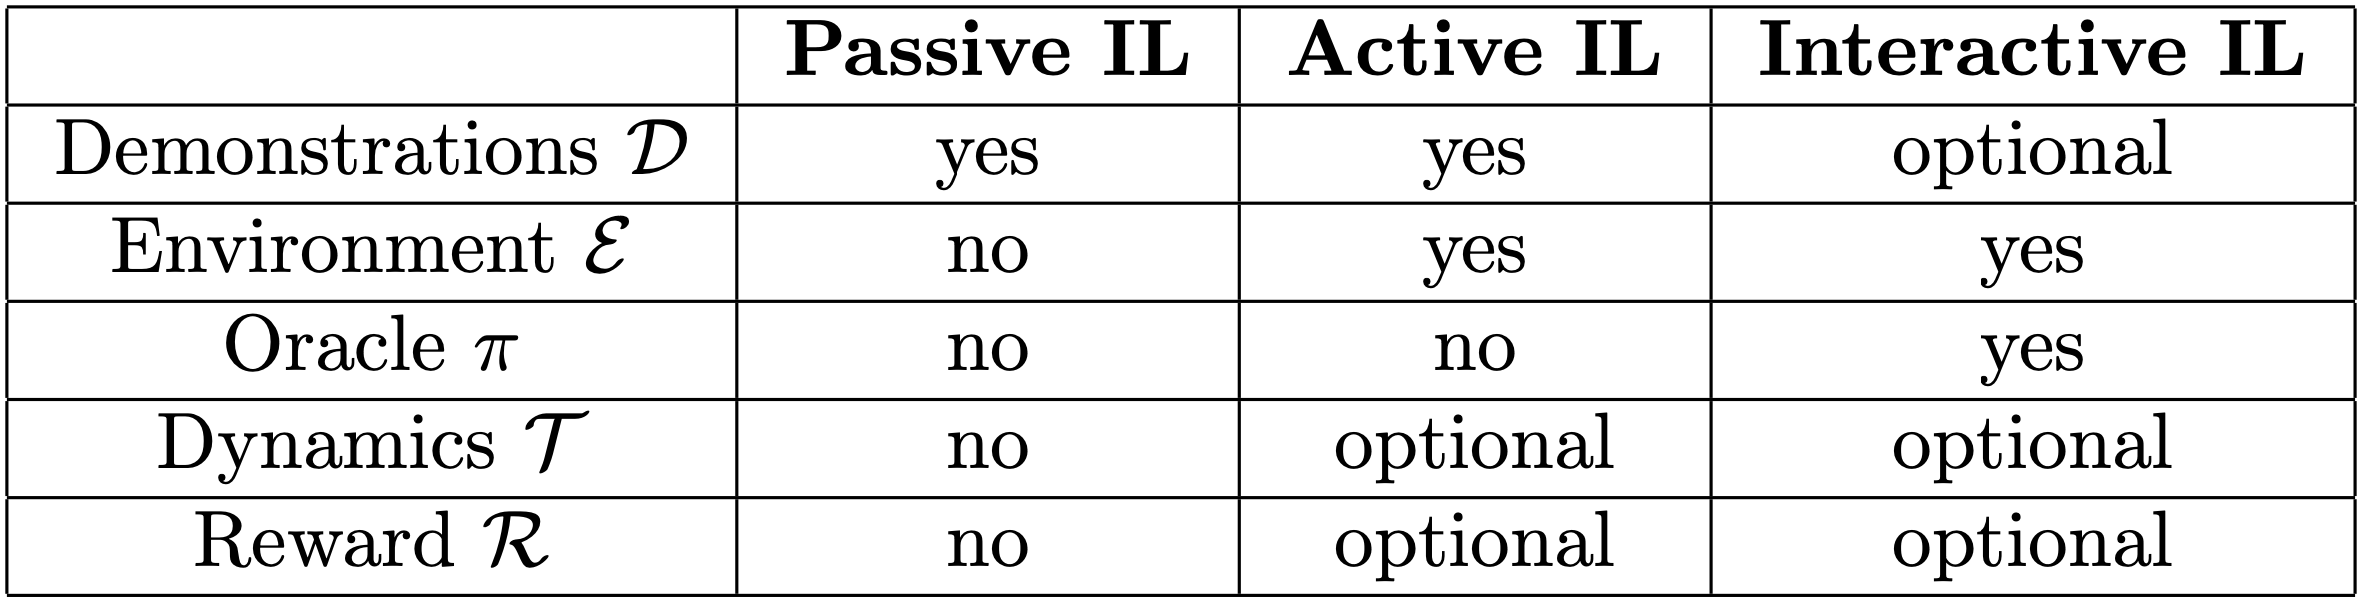
\includegraphics[width=0.7\textwidth]{images/3IL.png}
    \caption{3 Types of Imitation Learning.}
    \label{f_3IL}
\end{figure}

\subsection{Passive IL}

\subsubsection{Problem Setup}

As we can observe from Figure~\ref{f_3IL}, passive IL sets a scenario where an agent only has access to demonstrations. The agent does not have access to the environment, and as such, it does not get any kind of feedback, nor has has access to the dynamics. 

One example of this type of IL, is behavioral cloning (supervised learning) shown in Figure~\ref{fig:passive}. In this paradigm, an agent gets expert demonstrations $\mathcal{D}^\ast = \{s_n, a_n\}_{n=1}^N$ which are passed through some sort of black-box (e.g. a neural network) from which we want to learn a function $\pi(a |s)$ representing (cloning) expert behavior.
\begin{figure}[H]
    \centering
    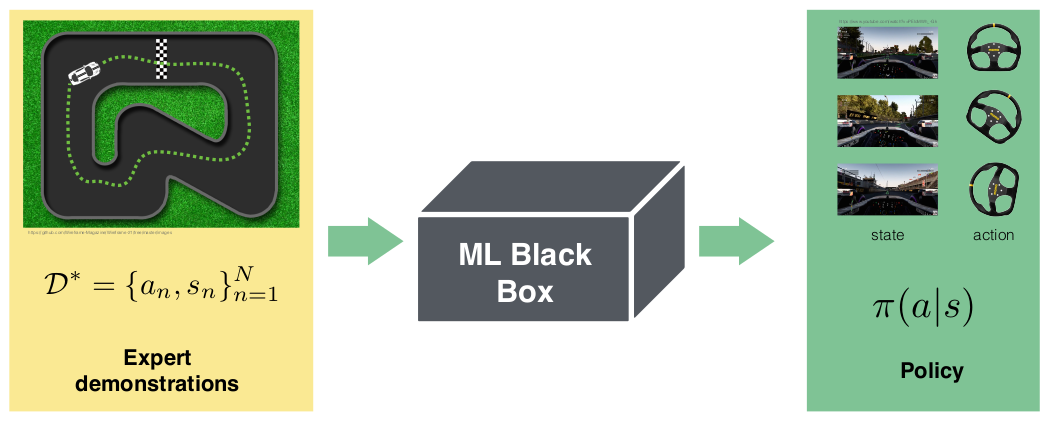
\includegraphics[width=0.7\textwidth]{images/passive_il.png}
    \caption{Passive IL.}
    \label{fig:passive}
\end{figure}

\subsubsection{Discussion}

Behavioral cloning suffers from covariate shift issues. At a high-level, covariate shift arises from having different test and training distributions. Now, since the agent (most likely) does not have data from all possible states, it can only model short-term behavior. Thus, we only train agents from current (short-term) inputs often lacking diversity. This may cause the agent to overfit to current inputs and is specially problematic in sequential problems where agents might accumulate small errors that ultimately lead to \textit{catastrophic} scenarios. 

For instance, imagine we train an agent to navigate on a road using this paradigm. Imagine the expert demonstrations only include driving "perfectly" straight, and thus, the agent is only shown that type of behavior. The agent in this scenario will learn to \textit{always} navigate straight. However, if at some point the agent starts accumulating errors by steering slightly less straight (or because it has to turn and it has not learned to do so) this could eventually lead the agent to a set of states which it has never seen. Thus, in not knowing how to respond to such unknown set, the agent might end up in a state from which it might not be able to recover, like crashing into a wall. 

\subsection{Interactive IL}

\subsubsection{Problem Setup}

As mentioned above, one potential problem of Passive IL is that it only models short-term (one-shot) behavior. During test, the agent is likely to get into unseen states with accumulation of small errors. Unless there are data from all states, the problem still remain. Moreover, collecting enough data is challenging because data with negative label (e.g. samples lead to crash) are rare.

To solve the problem, we introduce Interactive IL. Compared with Passive IL, Interactive IL has the ability to interact with the environment, i.e. it executes current policy and queries experts to get feedback. We will introduce two Interactive IL algorithms DAgger and AggreVaTe in the following.

\subsubsection{DAgger}
DAgger (Data Aggregation) \cite{ross2011reduction} is proposed to solve two main problems of IL: data dependencies (not i.i.d.) and errors accumulation. Figure \ref{f_dagger} illustrates the framework of DAgger and Algorithm \ref{algo:dagger} shows the pseudo code of DAgger. It first mixtures policy between expert policy and hindsight optimal policy, then samples state-action pairs using mix policy from the environment. DAgger aggregates all sampled states with former data and update the hindsight optimal policy via minimizing the zero-one loss function. 

\begin{algorithm}[H]
\caption{DAgger}
\label{algo:dagger}
\begin{algorithmic}[1]
\FOR{$k=1,\;\cdots,\;K$}
\STATE $\pi_k \triangleq \beta\pi^* + (1-\beta)\hat{\pi}_k$
\STATE $\{s^{(t)},a^{(t)}\}_{t=1}^T\sim\varepsilon|\pi_k$
\STATE $\mathcal{D}\leftarrow\mathcal{D}\cup\{s^{(t)}\}_{t=1}^T$
\STATE $\hat{\pi}_{k+1}=\arg\min_{\pi\in\Pi}\sum_{d=1}^{|\mathcal{D}|}f(\pi(s^{(d)}),\pi^*(s^{(d)}))$
\ENDFOR
\RETURN $\hat{\pi}$
\end{algorithmic}
\end{algorithm}

Recall the general framework for Online Learning where the online learner updates parameters according to the obtained loss from the nature in each iteration, we notice that Interactive IL can be solved with the FTL (Follow-The-Leader) algorithm and DAgger is just FTL algorithm which is no-regret given a convex loss function. 

DAgger addresses domain shift problem by sampling trajectories which implicitly accounts for sequential dependence of actions and reduces IL to online learning results in no-regret bounds. However, it solves for each iteration for the optimal policy which is costly and treats all mistakes equally.

\begin{figure}[H]
    \centering
    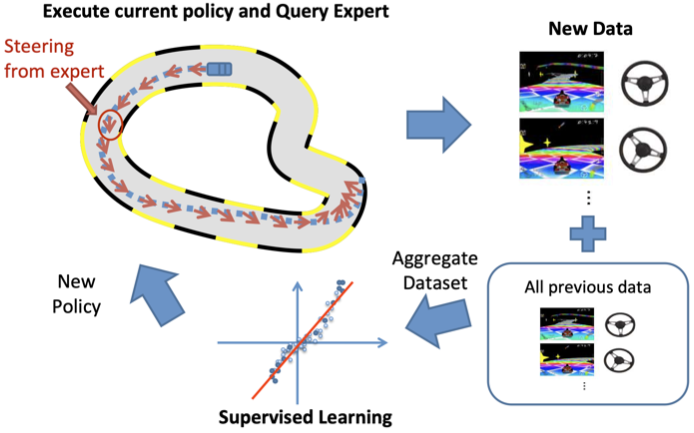
\includegraphics[width=0.7\textwidth]{images/DAgger.png}
    \caption{Illustration of DAgger.}
    \label{f_dagger}
\end{figure}

\subsubsection{AggreVaTe}
DAgger minimizes the number of mistakes of the learned policy compared to expert and treats all mistakes equally. In reality, mistakes are different, some mistakes can be recovered while others may be fatal. We would like to improve DAgger to assign different penalties to different mistakes. 

AggreVaTe (Aggregate Values to Imitate) \cite{ross2014reinforcement} is proposed to overcome DAgger's deficiencies. Algorithm \ref{algo:aggrevate} shows the pseudo code of AggreVaTe. Firstly, it follows the aggregated policy $\pi_k$ and stop at a random time step $t$. Then it takes each exploratory action and follows expert policy $\pi^*$ to obtain cumulative cost from the expert. After that it aggregates the state and cumulative cost into a cost sensitive dataset, indicating different weights of predictions, implying that some mistakes are more costly. AggreVaTe loops this procedure by resetting the state and recording all the cost Q values. Different from DAgger, AggreVaTe uses Q function as loss function, it updates the optimal policy which minimizes the expert's cost-to-go.

\begin{algorithm}[H]
\caption{AggreVaTe}
\label{algo:aggrevate}
\begin{algorithmic}[1]
\FOR{$k=1,\;\cdots,\;K$}
\STATE $\pi_k \triangleq \beta\pi^* + (1-\beta)\hat{\pi}_k$
\STATE $t_k\sim[T]$
\STATE $\{s^{(i)}\}_{i=0}^{t_k}\sim\varepsilon|\pi_k$
\STATE $\mathcal{D}\leftarrow\mathcal{D}\cup\{s^{(t)},Q(s^{(t_k)})\}_{t=1}^T$
\STATE $\hat{\pi}_{k+1}=\arg\min_{\pi\in\Pi}\sum_{d=1}^{|\mathcal{D}|}\sum_a\pi(a|s_d)Q^*(s_d,a)$
\ENDFOR
\RETURN $\hat{\pi}$
\end{algorithmic}
\end{algorithm}

\subsubsection{Conclusion}
The difference between DAgger and AggreVaTe can be summarized as follows:
\begin{itemize}
    \item DAgger treats all the mistakes equally while in AggreVaTe some mistakes are worse (fatal) than others (can be recovered).
    \item AggreVaTe asks expert the consequence of mistakes (i.e. Q function) rather than the correctness of the action.
    \item AggreVaTe minimizes the cost of mistakes made by the policy instead of the number of mistakes the policy make.
\end{itemize}

Since the data are sequential (not i.i.d.), traditional statistical learning tools are not ideal for understanding analyzing sequential decisions. To analyze sequential decision making problems, online learning with no-regret analyses would be a proper choice. Imitation and reinforcement learning enable super-expert performance. Imitation learning avoids global exploration, thus it is more sample efficient.

\section{Wrap-Up}

This section serves as a brief summary of the content discussed in this course. 

\subsection{Hitchhiker's guide to RoboStats}

The goal of \textit{16-831 Statistical Techniques in Robotics} was to provide a theoretical introduction for decision making and statistical learning approaches that are commonly used in robotics. The course is mainly focused in modeling data driven sequential decision processes, and in particular, this course followed (in the order indicated by the arrows) the topics outlined in the Figure~\ref{fig:robostats}.

\begin{figure}[H]
    \centering
    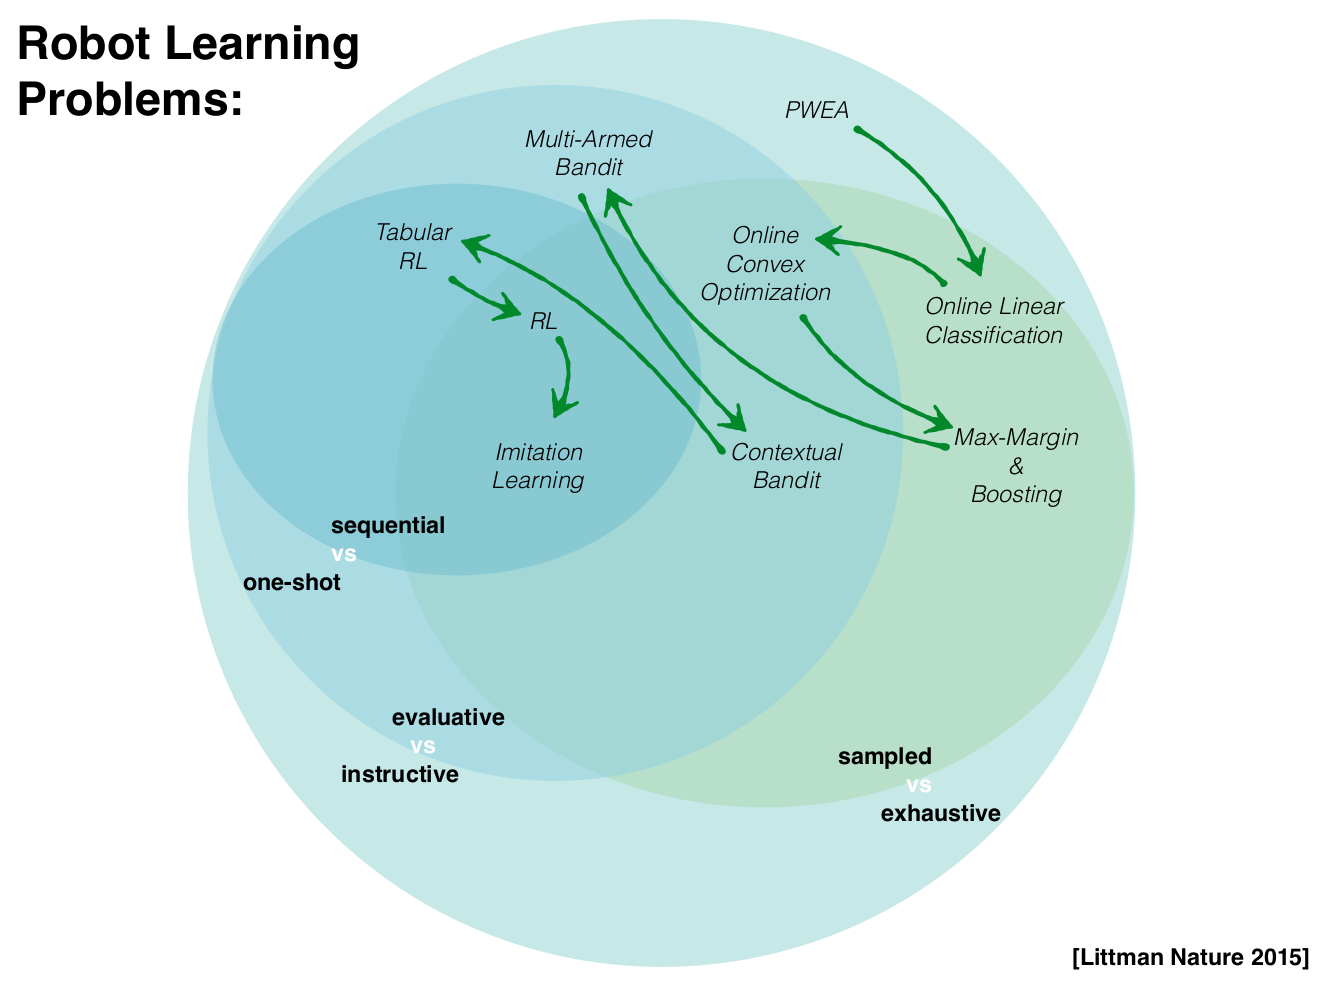
\includegraphics[width=0.7\textwidth]{Scribe_template/images/robostats.png}
    \caption{Statistical Techniques in Robotics}
    \label{fig:robostats}
\end{figure}

We started off the class by setting up the problem that a robot system requires to operate and learn under different conditions and it is up to us, the algorithm designers, to understand such problem settings and its appropriate solutions. To do so, we need to know what type of feedback do we get from the environment(s) our agents interact with. For this reason, we defined three questions to guide ourselves in making a decision as to what type of approach to use in a given problem:
\begin{enumerate}
    \item Does the \textbf{learner} get to see all the data?
    \begin{itemize}
        \item \textit{Exhaustive feedback.} The learner gets exposed to all possible situations (e.g., tabular reinforcement learning).
        \item \textit{Sample feedback.} The learner only gets to access a subset of the situations (e.g, online linear classification).
    \end{itemize}
    \item What kind of \textbf{feedback} do we get from the \textbf{environment}?
    \begin{itemize}
        \item \textit{Evaluative feedback.} The learner does not have information for all alternative actions (e.g., reinforcement learning, imitation learning algorithms)
        \item \textit{Instructive feedback.} The learner receives a score for all actions possible (e.g., prediction with expert advice)
    \end{itemize}
    \item Is \textbf{feedback} sequence dependent?
    \begin{itemize}
        \item \textit{Sequential feedback.} The learner's current action affects the future state/action (e.g., reinforcement learning, imitation learning).
        \item \textit{One-Shot feedback.} The learner's current action does not affect the next action (e.g., bandits).
    \end{itemize}
\end{enumerate}

For reference, the following list includes all the algorithms covered during class:
\begin{multicols}{2}  
\begin{enumerate}
    \item \textbf{Prediction with Expert Advice}
    \begin{itemize}
        \item Greedy
        \item Randomized Greedy
        \item Majority
        \item Weighted Majority
        \item Randomized Weighted Majority 
    \end{itemize}
    \item \textbf{Online Classificaton}
    \begin{itemize}
        \item Perceptron
        \item Winnow
        \item SVM
        \item AdaBoost
    \end{itemize}
    \item \textbf{Multi-Armed Bandits}
    \begin{itemize}
        \item Upper Confidence Bound
        \item Thompson Sampling
        \item EXP3
        \item EXP4
    \end{itemize}
    \item \textbf{Online Convex Optimization}
    \begin{itemize}
        \item Follow the Leader
        \item Follow the Regularized Leader
        \item Online Gradient Descent
        \item Online Mirror Descent
    \end{itemize}
    \item \textbf{Reinforcement Learning}
    \begin{itemize}
        \item Policy Iteration
        \item Value Iteration
        \item TD Control
        \item Monte-Carlo Control
        \item Value Approximation
        \item Policy Gradient
        \item Actor-Critic
    \end{itemize}
    \item \textbf{Imitation Learning}
    \begin{itemize}
        \item Linear Program IRL
        \item Game Matrix IRL
        \item Max Margin IRL
        \item Structured Max Margin IRL
        \item Max Entropy IRL
        \item GAIL
        \item DAgger
        \item AggreVate
    \end{itemize}
\end{enumerate}
\end{multicols}
 
%\section*{References}
%Include your references here. Please cite any resources you found useful.	
%Populate the refs.bib file or list your references manually. Be consistent in formatting!
{
\bibliography{refs}
\bibliographystyle{abbrv}
}

%\section{Appendix}
%This section provides any relevant background material that was not covered in the lectures, but was found to be useful for understanding the material. 
%For example, derivations, theory underlying techniques employed, etc. 

%Additionally, this section can summarizes applications or extensions of these techniques found in the literature. 

\end{document} % Done!


